\documentclass{article}
\usepackage[utf8]{inputenc}
\usepackage[english]{babel}
\usepackage{multicol}
\usepackage{natbib}
\usepackage{graphicx}
\usepackage{float}
\usepackage{amsfonts}
\usepackage{amssymb}
\usepackage[bottom]{footmisc}
\usepackage{listings}

\begin{document}

\begin{titlepage}

    \center
    
    
\includegraphics[scale=0.5]{AzuGryphonSharp.png} %\vspace{0.5cm}
    
    \huge  \textbf{GryphonSharp Proposal}
    
    \vspace{2cm}
    
    \Large \textbf{Azureus Aeterna, kilanth@icloud.com}
    
    School of Computing and Communications
    
    Lancaster University
    
    \vfill
    
    Coordinator: Abe Karnik (a.karnik@lancaster.ac.uk)\endgraf
    Research group: Human Computer Interaction
    
    \end{titlepage}
\pagebreak


\section{Introduction}
Recently, world has been heavily digitized - practically, every aspect of everyday life is in digital form ranging from digital watches to entire industries \citep{jovanovi_digitalization}. With the increasing demand for programming in nearly all science disciplines, need for programming education has risen drastically \citep{MargGoodBern2011wv, jovanovi_digitalization, 7318200}.
Before long, computers were mere 'calculators' which were able to perform straightforward computational tasks with ease. For example multiplying big numbers or computing root, power and other mathematical functions. At the time, the only human-understandable language which could be easily understood by a computer was - Assembly.
Assembly language was and is one of the hardest computer languages to read and understand, it's built on a 'one-at-the-time instruction' basis and translates directly into machine code that the computer can then execute. Programming in this language would require a lot of patience, as even simplest programs that display 'Hello World!' would require significant time.
There was a strong need in development of the 'easily' understandable language that wider population can use to develop and build their programs. Such a language would require functionality that of Assembly, but also provide complementary metaphors as building blocks. Functionality simplification has been achieved through BCPL language. Later, C language featuring structs as the metaphor for building block, was derived from BCPL in early 1970s \citep{ritchie_the}.
Since the invention of C language, computer languages have been tremendous help in many applications. General purpose languages were introduced as help in development by complementing existing framework with standard building blocks and functionality in comparison to 'one-at-the-time instruction' assembly language.\citep{10.1145/364063.364092}
Languages evolved over time, 'higher' languages emerged as a result, for example Java or C\#. Unlike C, they provide not only building blocks, but ensure there are no errors before the code even compiles into lower languages, such as C or even directly assembler. However, users find even higher languages hard to use, especially minors. To address this and provide engaging education of programming and algorithmic thinking, Visual Programming Environment called 'Scratch, was introduced.\citep{1314376}

\section{Related Work}
Since introduction of Visual Programming Environments such as Scratch into education, average performance of students has increased \citep{tsai_2019_improving} while barriers of getting intuition in programming fell down \citep{kelleher_2005_lowering}. Researches \citep{7318200,tsai_2019_improving,kelleher_2005_lowering} clearly suggest visual environments have been tremendously helpful in education.
However, one of the unfortunate drawbacks of VPLs\footnote{Visual Programming Language-s} they are usually specifically designed.
E.g. Unreal Blueprints as shown in \ref{fig:blueprints}, were specifically designed to develop games or 3D-applications using the engine. This VPL is fairly easy to learn and use. Unfortunately, the scope of language is limited to the engine, and, further, to 3D applications. 

\begin{figure}[H]
\centering
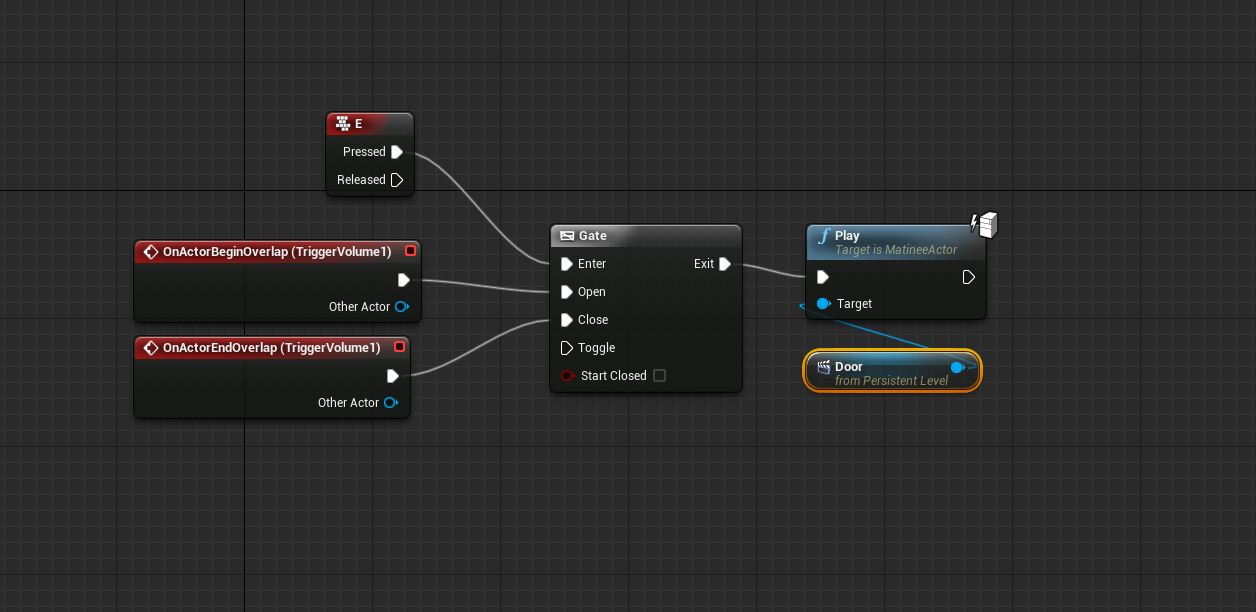
\includegraphics[width=1\textwidth]{0bfef1e3868153cc4b49a3dac0214b0d.jpg}
\caption{Unreal Blueprints}
\label{fig:blueprints}
\end{figure}

In another example, there is Scratch, which, was initially designed as an educational tool using Google's Blockly; now Scratch, or it's parent Blockly, can be accessed freely and used to develop JavaScript, Python and more\footnote{https://developers.google.com/blockly} code. Example Blockly code in figure \ref{fig:blockly} and it's compiled JavaScript version in listing \ref{jsout}.

\begin{figure}[H]
\centering
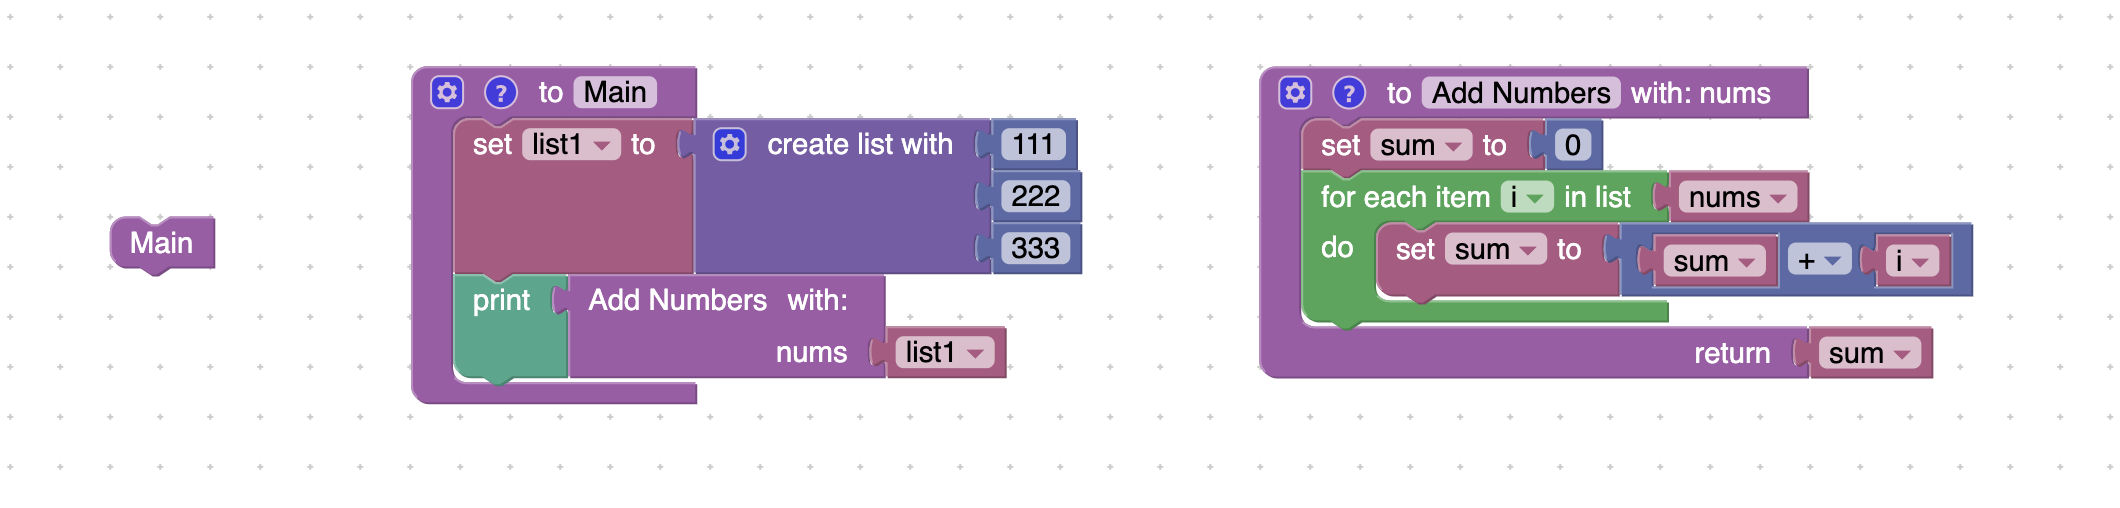
\includegraphics[width=1\textwidth]{Screenshot 2021-05-21 at 05.08.44.png}
\caption{Blockly example code}
\label{fig:blockly}
\end{figure}

\pagebreak

\begin{lstlisting}[frame=single, label=jsout, caption=Generated JavaScript Code]
  var nums, sum, list1, i;
  
  // Describe this function...
  function Main() {
    list1 = [111, 222, 333];
    window.alert(Add_Numbers(list1));
  }
  
  // Describe this function...
  function Add_Numbers(nums) {
    sum = 0;
    for (var i_index in nums) {
      i = nums[i_index];
      sum = sum + i;
    }
    return sum;
  }
  
  
  Main();
\end{lstlisting}


However, this is still highly limited as functionality has to be specifically defined by Blockly framework, as can be seen on figure \ref{fig:blockly}. On top of this, Blockly only provides variables and functions paradigms as can be seen here. There is no research that attempts to represent delegates, objects or anonymous paradigms (objects, classes, data) in Blockly.

On the other hand, a research \citep{10.1145/3364183.3364202} concludes promising results of VPL usage in the industry. There participants were asked to construct a deep learning model with VPL (see figure \ref{fig:dl-ide}) and a traditional language. There VPL performed with flying colors. This research strongly suggests VPLs are the future of coding.

\begin{figure}[H]
\centering
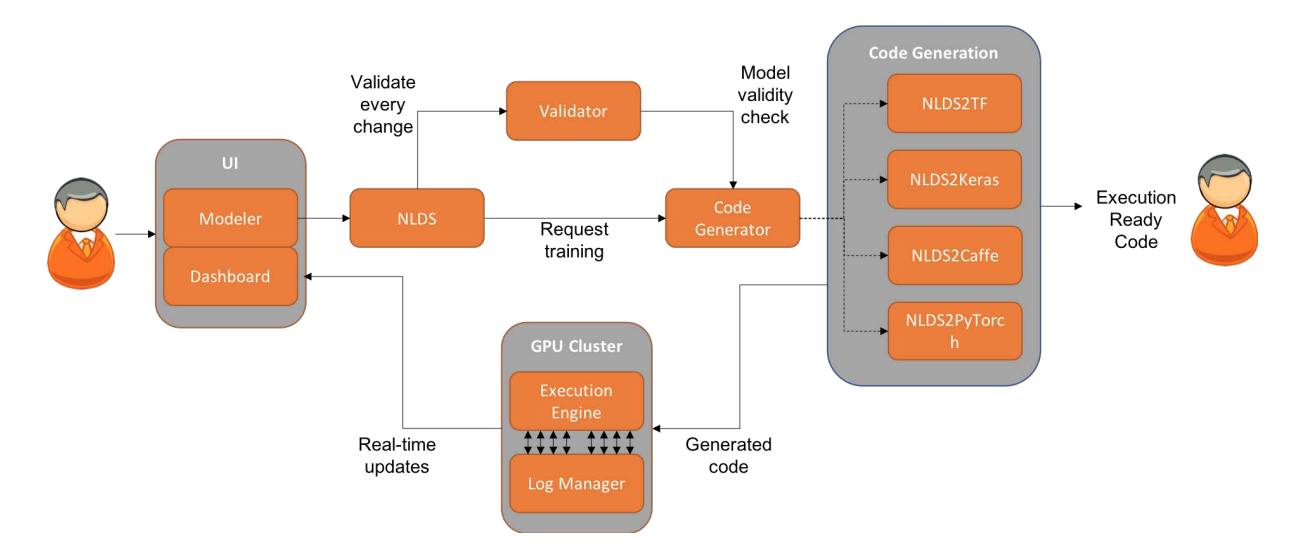
\includegraphics[width=1\textwidth]{Screenshot 2021-05-21 at 06.02.17.png}
\caption{Architecture and Components of DL IDE}
\label{fig:dl-ide}
\end{figure}

The research \citep{10.1145/3364183.3364202} clearly suggests VPL can be used in the industry and proved to be effective. This begs a question: Is code quality affected by the language? A study \citep{5298423} on bugs of Mozilla through Bugzilla database, discovered clear relation between density of bugs and languages that were used (C, C++ and Java). Safest language, and therefore highest, Java has achieved near 0 critical bug severity, in comparison to C languages without Type-safety, Java Virtual Machine abstraction and other features of Java language.

\section{Scope}
Project will cover basic programs without extensive programming features, such as attributes, abstraction or even basic objects. The aim here is to fuse already existing studies of visual programming languages into a working prototype that is capable of producing simple programs, such as "guess a number" or "console calculator".
The prototype will be 100\% operational and compile directly into C\#. This means, the node editor will be able to save visual representation in source files, which will be then picked up by transpiler.

\section{Methodology}
\subsection*{Overview}
Implementing fully functioning programming language that compiles into assembler is a genuinely time-consuming task, which also requires in-depth knowledge of different processor architectures such as ARM, AMD64 and Intel64. For this reason alone, timeframe will span over years and people\footnote{In comparison, C\# had years and years of evolution and development and has been greatly supported by Microsoft.}. In order to avoid building a bike from scratch by dropping thousands, if not millions, of hours of work put into development and optimization of C\#, the project's visual language will transpile into C\# Intermediate Language (henceforth IL) using CodeDOM feature of the language. IL is the common language, that is platform-independent, which can then be picked up by platform-specific runtime and executed.
\subsection*{Visual Editor}
The visual editor, or in this case node editor, will be implemented as a webpage canvas using Konvajs framework. Design of the node editor is the primary focus of the research.
Konvajs lets you easily serialize and deserialize data and populate the 'code map'. Refer to figure \ref{fig:codemap}.

\begin{figure}[H]
\centering
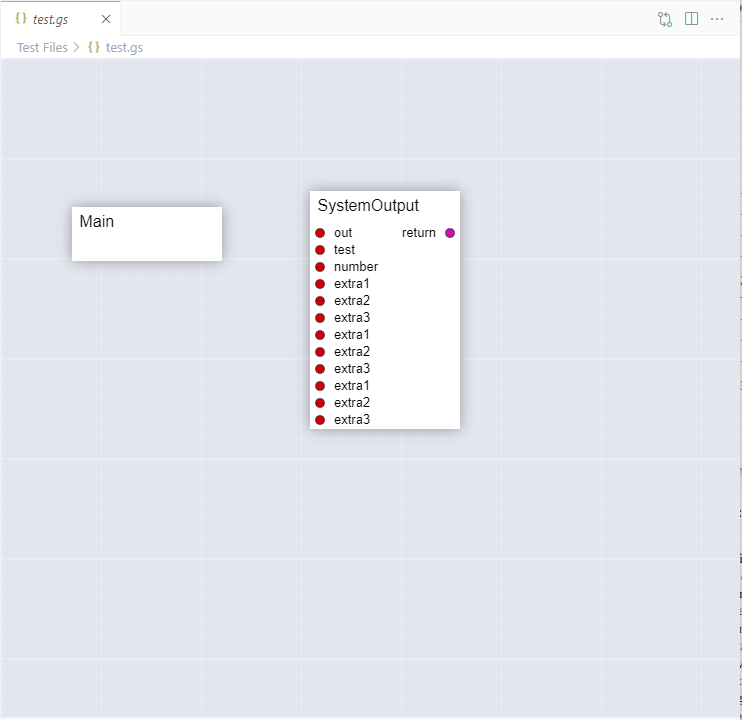
\includegraphics[width=1\textwidth]{codemap.PNG}
\caption{Code Map}
\label{fig:codemap}
\end{figure}

The webpage will be able to serialize all node structure into a JSON file, which will be a source code of a file. This JSON can then be parsed by Transpiler and convert its contents into C\# IL.
The Konvajs framework will be closely tied with Electron app called 'Visual Studio Code' (henceforth VSCode). VSCode is a ready-to-use out-of-the-box solution for any programming task in most if not all existing programming languages out there. VSCode has rich API for developing extensions and already defines great features to support custom languages, web-views and more\footnote{https://code.visualstudio.com/api}.
\subsection*{Transpiler}
As previously stated, the primary purpose of a transpiler is converting source of GryphonSharp-generated JSON files into C\# IL. CodeDOM feature is particularly good for the job, because it contains factories that could be used to allow compilation into, potentially, any other language. For example, CodeDOM out-of-the-box can compile into C\# and IronPython.
\subsection*{Language Server}
Language Server has a sole purpose of communicating with another language server 'Omnisharp'. Omnisharp is a language server that allows resolving types, extract compiled metadata and provide some syntax checking with autocompletion suggestions. It's obvious, language server is a necessary tool for any language, here Omnisharp plays that exact role.
However, custom language server would be required to account for non-standard language features that might emerge as a result of this research, such as different data management design (in comparison to C\#'s object-oriented design).

\section{Time Plan}
Project's time plan will span over 3 months and is represented by Gantt Chart below \ref{fig:gantt}.

\begin{figure}[H]
\centering
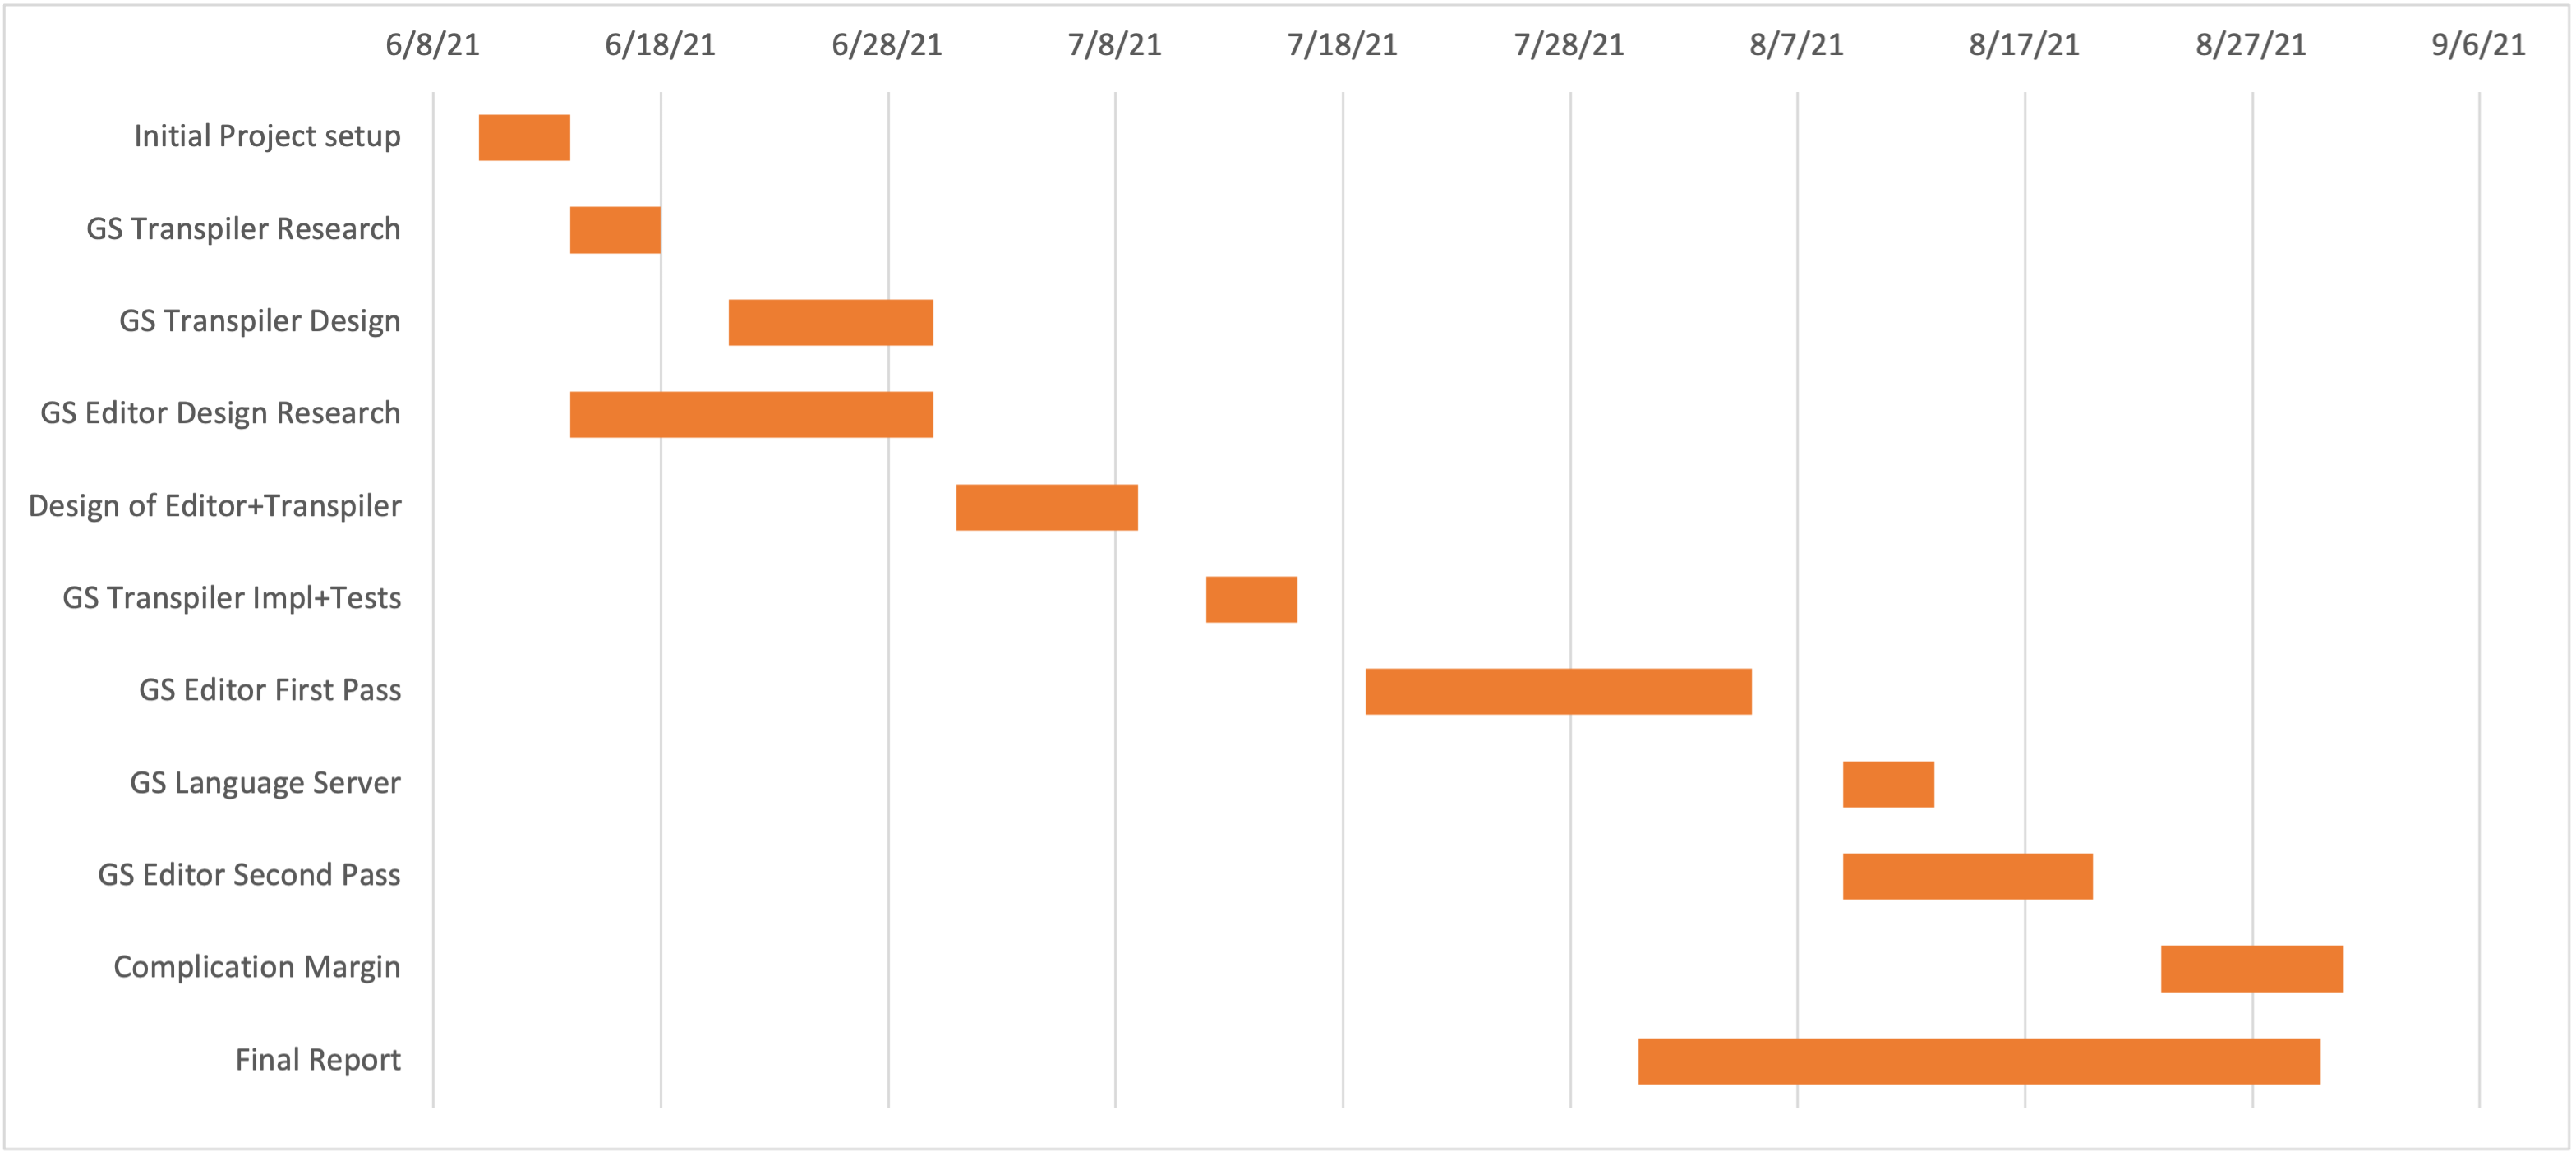
\includegraphics[width=1\textwidth]{Gantt.png}
\caption{Gantt Chart}
\label{fig:gantt}
\end{figure}

\section{Summary}
The project proposes to make in-depth research of current state of Visual Programming Technologies and compile a prototype, based on that research.
At the end of the research, fully functional prototype is expected. Functionality of prototype is defined in section Scope.

Prototype will come in multiple flavors: 
\begin{itemize}
  \item \textbf{Node Editor} - visual editor produces JSON source code files.
  \item \textbf{Transpiler} - takes JSON source files and converts them into CLR\footnote{Common Runtime Language: https://docs.microsoft.com/en-us/dotnet/standard/clr}.
  \item \textbf{Language Server} - helps \textbf{Node Editor} with suggestions, errors and more\footnote{More in section on Language Server}.
\end{itemize}



\bibliographystyle{plain}
\bibliography{refs}
\end{document}
